\section{Numerical evidence and transportation interpretation}\label{sec:numerics}
Sioux Falls absolute accounts use benchmark flows in veh/h and time units of $0.01$ h; multiply an account by $0.01$ for the hourly vehicle-hour total. Anaheim uses vehicle-minutes per hour. All experiments use the stated fixed-path logit-SUE assignment models and prespecified demand scenarios; shares reported over boundary families are enumeration shares over those families. The adaptive reporting rule of Section~\ref{sec:stability} organizes the experiments: every query either receives one error-controlled common value or an explicit spatial profile. The subsections examine, in order, how that selection varies across demand and congestion regimes, which traffic mechanisms generate the spatial variation and how stable they are under alternative attribution paths, and what complete profiles with compact summaries look like on a large network.

\subsection{Adaptive summary selection across demand and congestion regimes}\label{sec:adequate}
Sioux Falls has 24 nodes and 76 arcs in one block atom. Its structural weight condition is therefore the same for every OD, and the connected and unrestricted classifications coincide; the experiments measure variation due to realized responses and heterogeneous marginal costs. The query-dependent classification is illustrated separately in Figure~\ref{fig:blockcut}.

Six input-selected queries away from node 10 change jointly from $0.2$ to $1.6$ times their base values with all other demands fixed and routes responsive; they are the shortest and longest free-flow ODs in each demand tercile (Appendix~\ref{supp:newod}). Table~\ref{tab:newod} reports their ranges. The adaptive rule separates them sharply: the geometric accounts for $(7,18)$ lie in $[642,702]$, their midpoint $672$ has maximum absolute error $30$, or $4.3\%$ of the largest account, and this family admits one common summary at a $5\%$ tolerance; the $(1,19)$ and $(7,12)$ geometric ranges cross zero and require boundary-specific reporting at every tolerance considered below.
\begin{table}[pos=htbp]
\footnotesize
\caption{System contributions and spatial ranges for six prespecified queries,
setting C (TSTT units). Connected: all admissible connected regions;
screenline: the geometric family constructed independently of attribution
values. All $C_j$ are positive. Origin-cut accounts, negative shares, and
neighbourhood ranges are retained in Appendix~\ref{supp:newodaccuracy}.}
\label{tab:newod}
\small
\begin{tabular*}{\tblwidth}{@{\extracolsep{\fill}}lrrr}
\toprule
OD & $C_j$ & Connected [min, max] & Screenline [min, max]\\
\midrule
$(7,18)$ & $672.9$ & $[634{,}\ 710]$ & $[642{,}\ 702]$ \\
$(1,19)$ & $50{,}097.7$ & $[-13{,}502{,}\ 24{,}260]$ & $[-2{,}767{,}\ 22{,}124]$ \\
$(4,5)$ & $2{,}826.0$ & $[2{,}396{,}\ 3{,}452]$ & $[2{,}652{,}\ 3{,}176]$ \\
$(1,15)$ & $77{,}403.2$ & $[-8{,}286{,}\ 40{,}540]$ & $[511{,}\ 36{,}621]$ \\
$(6,8)$ & $73{,}964.9$ & $[35{,}307{,}\ 66{,}695]$ & $[45{,}230{,}\ 65{,}286]$ \\
$(7,12)$ & $117{,}482.3$ & $[-17{,}616{,}\ 60{,}029]$ & $[-2{,}967{,}\ 57{,}780]$ \\
\bottomrule
\end{tabular*}
\end{table}

Experiment C widens the view to an input-only selection of 18 of the 528 positive Sioux Falls OD demands, taking two lexicographically predetermined positions from each demand-by-free-flow-time tertile cell. Each OD changes alone over $\pm10\%$ and $\pm20\%$ intervals while other demands remain fixed with endogenous rerouting; the same 36-direction geometric family is used throughout, and Appendix~\ref{sec:coverage} reports every query and both widths. For each nonempty family, let $\beta=(\phi_{\max}+\phi_{\min})/2$ and $\varepsilon=(\phi_{\max}-\phi_{\min})/2$. This common summary minimizes the largest absolute discrepancy, so every reported boundary satisfies $|\phi(U)-\beta|\leq\varepsilon$. The reported normalized error is
\begin{equation}
r_j^{\mathcal F}=100\,\varepsilon_j^{\mathcal F}\Big/\max\bigl(|\phi_{j,\min}^{\mathcal F}|,|\phi_{j,\max}^{\mathcal F}|\bigr),
\label{eq:normerror}
\end{equation}
the absolute deviation of every account from the common value as a
percentage of the family's largest account magnitude; it does not bound
each account's own relative error. We apply a fixed descriptive tolerance
$r_j^{\mathcal F}\leq5\%$; this is a reporting choice rather than a
transport welfare threshold. When all accounts in a family share one
sign, $r_j^{\mathcal F}\leq50\%$, so values near $50\%$ indicate that
the smallest magnitude is far below the largest, not that the accounts
nearly agree.
At $\pm10\%$ and $\pm20\%$, respectively, 1 and 1 of 18 queries meet this tolerance, while 1 and 1 have accounts of both signs; representative common summaries at $\pm20\%$ appear in Appendix~\ref{sec:coverage}.

\begin{figure}[t]\centering
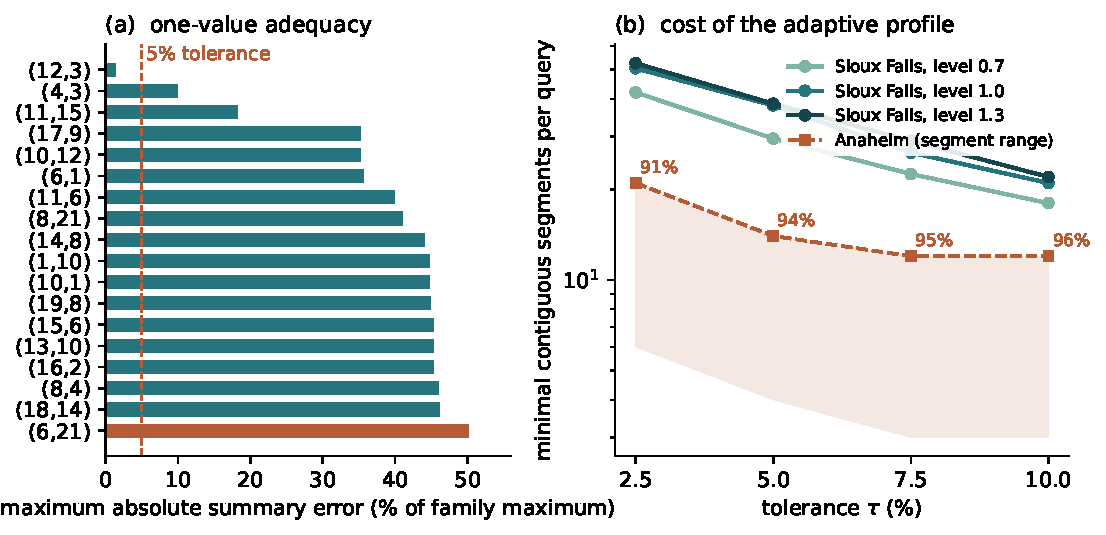
\includegraphics[width=0.99\linewidth]{../figures/fig_v107_summary_frontier.pdf}
\caption{Adaptive summary selection and its cost. Left: maximum absolute
summary error (Eq.~\eqref{eq:normerror}) over all 18 input-stratified
queries at $\pm20\%$, with the queries reordered by error; the $5\%$
tolerance marks which queries receive one common value. Right: the
alternative output --- median minimal contiguous segments per query on
Sioux Falls (of a median 86.5 family regions, three load levels) and
per-query segment ranges with compression on Anaheim --- as the
tolerance varies from $2.5\%$ to $10\%$; underlying numbers in
Table~\ref{tab:tolerance} (Appendix~\ref{sec:coverage}).}\label{fig:commonsummary}\end{figure}

Figure~\ref{fig:commonsummary} presents the selection and its cost. A minority of queries admits one common value at a working tolerance, and the remaining queries are represented by few position-adaptive segments with strict error control: relaxing the tolerance from $2.5\%$ to $10\%$ keeps the number of Sioux Falls queries admitting a single common value between zero and two at every load level, while the median number of contiguous segments per query falls from 42--53 to 18--22 of a median 86.5 family regions; on Anaheim's ordered families the same relaxation raises the compression of the 83--211 accounts per query from $91.5\%$ (6--21 segments) to $96.4\%$ (3--12 segments). With the same segment count, equal-count partitions have median worst-segment error $2.7$--$10.4$ times the tolerance on Sioux Falls and $4.7$--$18.8$ times on Anaheim, so position-aware segmentation is what buys the error control, not the segment count alone.

The $\pm10\%$ and $\pm20\%$ summaries of the same 18 queries are close in normalized terms, so further subdividing the perturbation width adds little information. The congestion state of the baseline is the more informative axis. All 528 demands are scaled jointly to $0.7$, $1.0$ and $1.3$ times their published values; at each level the level equilibrium is solved once, the focal query alone moves by $\pm20\%$, other demands stay fixed with responsive routes, and the endpoint identity supplies the attribution column (solver protocol in Appendix~\ref{supp:newod}).
\begin{table}[t]\centering\footnotesize
\caption{Common-summary statistics across baseline load levels (18
queries, focal $\pm20\%$, same 36-direction family). Normalized error
is Eq.~\eqref{eq:normerror}; the ratio column is the median
geometric-to-unrestricted spread ratio.}\label{tab:loadlevels}
\begin{tabular}{rrrrrr}\toprule
Level & Queries within $5\%$ & Mixed signs & Median error (\%) & Median ratio & Max.\ negative share\\\midrule
$0.7$ & 2 & 0 & 34.5 & 0.529 & $0.00\%$\\
$1.0$ & 1 & 1 & 44.4 & 0.574 & $0.67\%$\\
$1.3$ & 0 & 3 & 45.2 & 0.563 & $4.03\%$\\
\bottomrule\end{tabular}\end{table}
Table~\ref{tab:loadlevels} shows a monotone pattern: under the light
baseline, accounts are flatter across the family --- the median
normalized error falls to $34.5\%$, two queries satisfy the $5\%$
tolerance and no family crosses zero --- whereas the heavy baseline
makes every query exceed the tolerance, three families mix signs and
the negative share of $(6,21)$ reaches $4\%$. Per-query normalized
errors rise from the light to the heavy level for 17 of 18 queries
(e.g.\ $(10,12)$: $18.6\to35.2\to40.3$; $(1,10)$: $31.2\to44.8\to48.0$).
Across the load levels, light-load conditions admit transferable single
summaries more often, and heavy-load conditions require
boundary-specific reporting. The load-level trend has a theory-side
counterpart: the node-imbalance norm $\norm{d_j}_2$ rises by a factor
of $13.2$ from the light to the heavy baseline, and Eq.~\eqref{eq:cutspread}
sums that imbalance into the spatial range
(Appendix~\ref{sec:coverage} reports the rank correlations and the
Cauchy--Schwarz comparison).

\paragraph{How much does the model-specific level buy?}\label{sec:levelsdiag}
The universal structural condition quantifies over all conservative
responses; Section~\ref{sec:levels} introduced the model-specific level
that reasons on the responses an assignment model can actually realize.
Table~\ref{tab:levelsdiag} evaluates the hierarchy numerically. On the
Figure-1 network with its published post-merge weights, the universal
condition fails because the off-path pendant atom is heterogeneous, yet
the model-specific tests hold exactly for the all-simple-paths
structure: every rerouting that model can make preserves the common
account, so restricting attention to realizable responses restores
transferability that the universal condition denies. On Sioux Falls the
two levels coincide --- the full-background fixed-path model spans the
complete circulation space through path exchanges, so its response
envelope contains every conservative response
(Appendix~\ref{supp:networks}) --- and both fail at realistic TSTT
weights, leaving the realized summaries of Table~\ref{tab:newod} as the
operative output. The diagnosis is stable across load levels: the
normalized universal violation stays within $2.08$--$2.21$ from the
$0.7$ to the $1.3$ baseline while $\rho_{\mathrm{swap}}$ falls from
$1.12$ to $0.80$ as congestion grows. On Anaheim the universal test
fails more decisively (normalized violation $10.08$) and the
model-specific test fails with it ($\rho_{\mathrm{swap}}=2.18$ over the
$404$-dimensional exchange space), so there too the realized layer
carries the reporting.
\begin{table}[t]\centering\footnotesize
\caption{Numerical diagnosis of the transferability hierarchy of
Table~\ref{tab:threequestions}. $\eta_{\mathrm{all}}$ and
$\eta_{\mathrm{conn}}$: weight spread within all atoms / within the
queried atoms, normalized by the mean weight. $\rho_{\mathrm{swap}}$:
weighted-divergence leakage of unit rerouting directions relative to a
unit reference response; $\rho_{\mathrm{swap}}=0$ certifies
$BDN=0$, and together with zero off-span residuals
$\rho_{\mathrm{ref},j}$ it certifies both conditions of the
model-specific level. On Sioux Falls (level $1.0$) three of the six
queries have $\rho_{\mathrm{ref},j}=0$; the other three lie in
$0.83$--$0.97$. Realized: median
normalized geometric common-summary error of the setting-C six
queries. Synthetic: published post-merge weights; Sioux Falls: TSTT
weights at the level-$1.0$ equilibrium, where the path-exchange space
attains the full circulation dimension $53$.}\label{tab:levelsdiag}
\begin{tabular}{lrrrr}\toprule
Network & $\eta_{\mathrm{all}}$ & $\eta_{\mathrm{conn}}$ & $\rho_{\mathrm{swap}}$ & Realized (\%)\\\midrule
Figure-1 synthetic & $0.61$ & $0$ & $0$ & $0$ (model responses)\\
Sioux Falls & $2.08$ & $=$ & $0.88$ & $32.3$\\
\bottomrule\end{tabular}\end{table}

\subsection{What generates spatial variation?}\label{sec:variation}
Experiment A varies the background treatment. Eight largest published OD demands, all incident to node 10, change jointly from $0.2$ to $1.6$ times their base values; every study OD has ten fixed paths. Settings A, B and C use zero background, frozen background link flows and fixed background demands with endogenous rerouting, respectively. Setting C assigns all 528 positive demands (full protocols in Appendix~\ref{supp:fields}).
Uniform weights provide a compatible control. The active-link outcome $T(F)=F_{10\to16}$ preserves the $(10,16)$ direction but permits a response-dependent scale; TSTT produces internal imbalance. Figure~\ref{fig:respfield} illustrates the three patterns on the same realized response: compatible weights give one common account on every boundary, the directional outcome balances along the OD but scales with the response, and TSTT weights generate genuine spatial structure. For its seed-zero TSTT response, expanding $\{10\}$ to $\{10,17\}$ lowers the account from $5.77\times10^4$ to $4.34\times10^4$, approximately $92\%$ of the unrestricted spread. The direct-SUE decrease is $24.80\%$ of its own origin-cut account (Appendix~\ref{supp:accuracy}). Both sides of these regions are connected. Free-flow weights explain $84.7\%$ of the node-17 imbalance: all incident links have free-flow time 2 except $10\leftrightarrow17$ with time 8, giving $[B\operatorname{diag}(t_0)G_j]_{17}=6(G_{10\to17,j}-G_{17\to10,j})$.
\begin{figure}[pos=t]
\centering
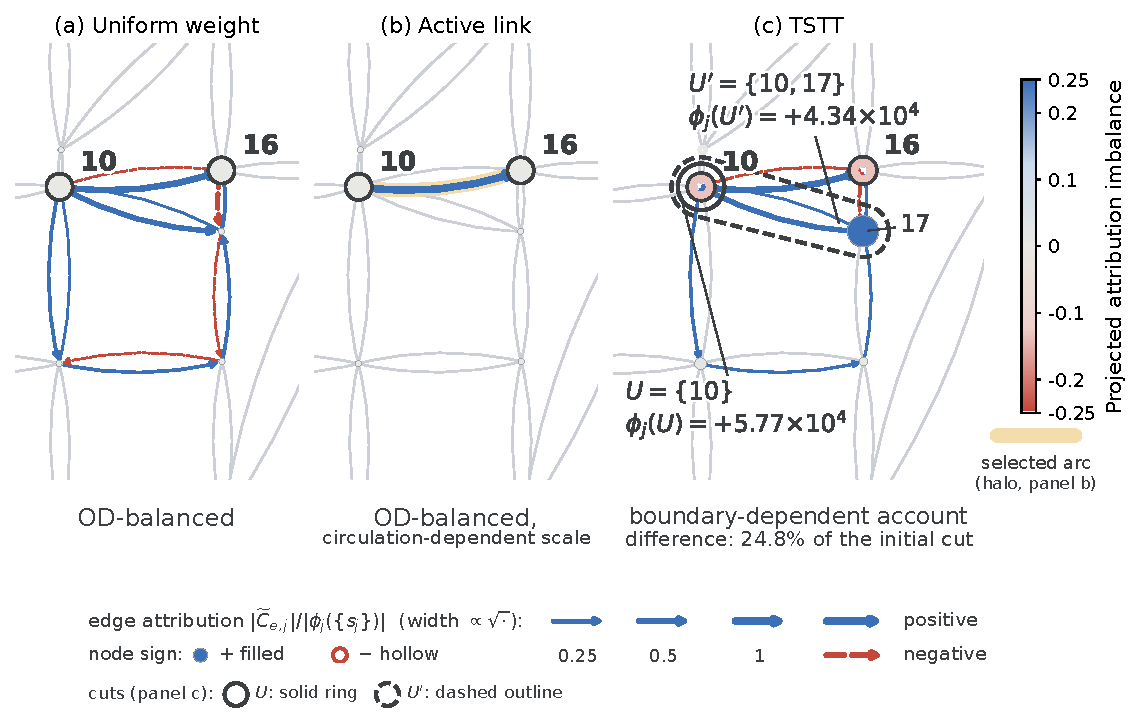
\includegraphics[width=0.9\linewidth]{../figures/fig_resp_field_v100.pdf}
\caption{OD $(10,16)$ endpoint attributions, zero background, learned
seed $0$. (a) Uniform weights give cut consistency. (b) The active-link
outcome balances in the OD direction but has no response-independent
scale. (c) The signed TSTT boundary account decreases by $24.8\%$ when
the boundary expands from $\{10\}$ to $\{10,17\}$. Widths encode
attribution magnitude; node colors show the projected attribution
imbalance $(d_j)_v$ (Eq.~\eqref{eq:endpointd}) divided by the absolute
origin-cut value.}
\label{fig:respfield}
\end{figure}

Table~\ref{tab:cutspreadperod} shows three representative queries of the eight under the three background settings (the complete table is in Appendix~\ref{supp:additional}); rerouting produces appreciable spatial variation for every query, and connected regions retain $60.41$--$76.85\%$ of the unrestricted range across the full set. Normalizations use each setting's own origin account: for $(17,10)$, the percentage falls from $59.95\%$ in A to $54.77\%$ in C while the absolute spread rises from 17,607.8 to 123,202.1, approximately sevenfold.
\begin{table}[pos=htbp]
\footnotesize
\caption{TSTT cut ranges as percentages of each account's absolute
origin-cut value; three representative queries shown, complete table in
Appendix~\ref{supp:additional}. A: zero background; B: frozen background
flows; C: background demands fixed, all traffic re-equilibrated. Learned
values are five-seed medians (ranges); all SUE columns are direct
($41$ quadrature points, implicit sensitivities).}\label{tab:cutspreadperod}
\small
\begin{tabular*}{\tblwidth}{@{\extracolsep{\fill}}lccccc}
\toprule
& \multicolumn{4}{c}{Unrestricted range (\%)} & Connected (\%)\\
\cmidrule(lr){2-5}\cmidrule(lr){6-6}
OD & Learned A & SUE A & SUE B & SUE C & SUE C\\
\midrule
$(17,10)$ & $59.71$ $(58.92$--$61.23)$ & $59.95$ & $56.38$ & $54.77$ & $35.27$ \\
$(16,10)$ & $36.80$ $(36.41$--$38.40)$ & $36.86$ & $39.99$ & $166.26$ & $127.72$ \\
$(11,10)$ & $0.18$ $(0.03$--$0.27)$ & $0.0073$ & $0.79$ & $81.09$ & $48.98$ \\
\bottomrule
\end{tabular*}
\end{table}
\paragraph{Same-state response decomposition.}\label{subsec:bgsplit}
Comparing A, B and C changes both costs and sensitivities. At each common setting-C state, split responses into study and background parts, with $BJ_j^{\mathrm{study}}=\mu_j$ and $BJ_j^{\mathrm{bg}}=0$. Weight both by the same total-flow TSTT gradient, yielding
\begin{equation}
\widetilde C_j^{\mathrm{tot}}=\widetilde C_j^{\mathrm{study}}+\widetilde C_j^{\mathrm{bg}}.
\label{eq:bg_attribution}
\end{equation}
At node 15 for $(10,16)$, study and background divergence contributions are $-973.1$ and $49{,}103.4$. Yet on the specified expansion $\{10\}\to\{10,17\}$, the account changes only $-3361.1$ ($-1305.0$ study, $-2056.1$ background), or $1.23\%$ of the initial account. Large extremal variation can coexist with similar selected accounts. Component differences add at a fixed region pair; their separate ranges do not add in general.

\paragraph{Free-flow and congestion mechanisms.}\label{subsec:newod}
For BPR costs, $g_e'=t_{0,e}+0.75t_{0,e}(F_e/c_e)^4$. Crossing these two weight terms with the two response terms gives four additive contributions, evaluated at identical states and the same reported boundary:
\[
\phi_j(U_-)=\sum_{a\in\{\mathrm{ff,cong}\}}\sum_{b\in\{\mathrm{study,bg}\}}\phi_j^{a,b},
\qquad \phi_j^{a,b}=-\Delta q_j\int_0^1\mathbf1_{U_-}^{\top}BD_\lambda^aJ_j^b(\lambda)\,d\lambda.
\]
Table~\ref{tab:ffcong} distinguishes the mechanisms behind the sign-crossing queries of Table~\ref{tab:newod}: study congestion dominates $(1,19)$, both congestion terms are negative for $(1,15)$, and background congestion dominates $(7,12)$. The combined free-flow contribution stays positive. The decomposition is additive at a common equilibrium state and identifies the contribution of each response--weight component.
\begin{table}[pos=htbp]
\caption{Four parts of the same boundary account at the reported
$U_-$ (setting C, six-query protocol; TSTT units; identical $41$-point
states, responses, and boundaries as Table~\ref{tab:newod}). Study
includes all six query ODs; background includes the other $522$.
Columns cross free-flow/congestion weights with study/background
responses. Entries are rounded independently.}\label{tab:ffcong}
\small
\begin{tabular*}{\tblwidth}{@{\extracolsep{\fill}}lrrrrr}
\toprule
OD & Free-flow study & Free-flow background & Congestion study & Congestion background & Total\\
\midrule
$(1,19)$ & $-361.3$ & $+759.0$ & $-17{,}357.9$ & $+3{,}458.6$ & $-13{,}501.6$ \\
$(1,15)$ & $+1{,}541.8$ & $+333.8$ & $-6{,}537.4$ & $-3{,}624.2$ & $-8{,}286.0$ \\
$(7,12)$ & $+3{,}897.0$ & $-1{,}311.1$ & $+125.5$ & $-20{,}327.6$ & $-17{,}616.2$ \\
\bottomrule
\end{tabular*}
\end{table}
The sign pattern itself is a spatial property, not a magnitude artefact. Negative accounts occupy $17.8\%$, $2.5\%$ and $7.3\%$ of the 14,477, 15,191 and 16,943 connected regions of the three sign-crossing queries. For $(1,19)$, the connected minimum $-13{,}501.6$ is attained on a 13-node region, whereas a 13-node free-flow neighbourhood has account $+10{,}756.0$: region size alone does not determine the account. At the minimizing boundary, outgoing attributions sum to $7{,}867.3$ and incoming attributions to $21{,}368.8$, so the signed crossing-link account is negative while $C_j=50{,}097.7>0$; Figure~\ref{fig:negmech} maps all 26 crossing links. Figure~\ref{fig:screenlines} shows the same contrast on two straight screenlines of the prespecified geometric family: the minimum and maximum screenline accounts of $(1,19)$ have opposite signs under one positive network-wide contribution.
\begin{figure}[pos=tb]
\centering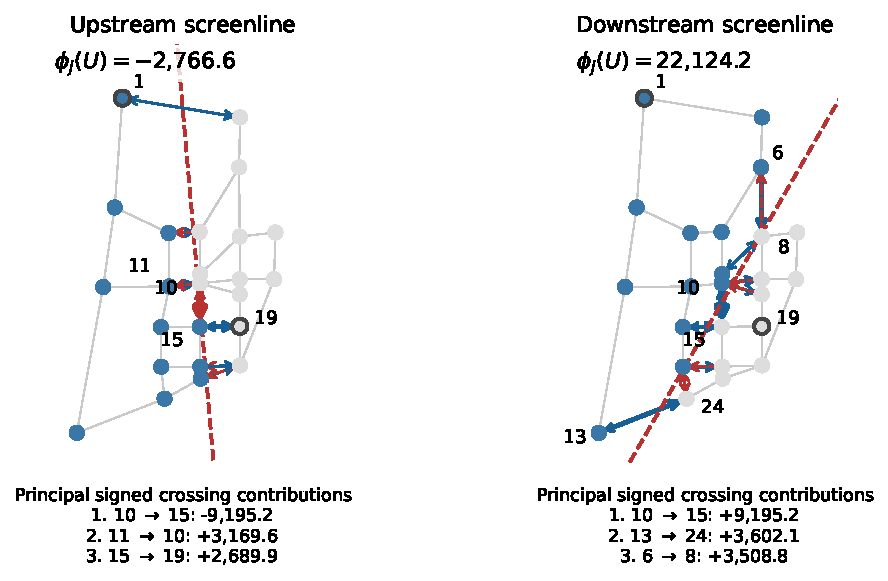
\includegraphics[width=0.64\linewidth]{../figures/fig_screenlines_v107.pdf}
\caption{Contrasting screenline accounts for the same positive OD
contribution. Two straight screenlines for OD $(1,19)$, setting C. Blue
nodes belong to $U$; grey nodes are outside; dashed lines separate the
two sides. Node $1$ is inside and node $19$ outside in both panels.
Upstream/downstream names the position of the separating line along the
corridor: its crossing progress with the straight origin--destination
segment is $0.61$ (left panel) versus $0.78$ (right panel). The two accounts have
opposite signs while the network-wide contribution is positive. The
lines are the minimum and maximum of the prespecified geometric family;
the complete irregular connected minimum and its crossing-link
decomposition appear in Figure~\ref{fig:negmech}.}
\label{fig:screenlines}\end{figure}
The straight-screenline family uses 36 directions at $5^\circ$ intervals, gaps between node projections, two-sided connectivity and duplicate removal; construction is independent of attribution. It contains 23--152 distinct regions per query. The $(1,19)$ and $(7,12)$ negative minima occur on 2/152 and 10/148 screenlines. Origin-centred hop and free-flow neighbourhoods remain positive but can differ in magnitude by factors 8.9, 9.0 and 3.4 for the three sign-crossing queries (Appendix~\ref{supp:newodaccuracy}). Sign stability and common-value accuracy are distinct properties.

\paragraph{Stability under alternative attribution paths.}\label{subsec:pathrobust}
With several ODs changing jointly, the per-query attribution columns
depend on the demand path; the columns are defined here under the
straight-line transition, and this paragraph quantifies that
dependence. Twenty-two piecewise-linear alternatives --- the six study
ODs changing one at a time, in canonical order, reverse order, and
twenty fixed-seed random permutations --- are compared with the
straight line on the setting-C protocol, with identical endpoints,
solver tolerance, quadrature and boundary family, and with the
mechanism decomposition evaluated at the same fixed regions $U_-$; the
total outcome change is path independent and reproduces to
$1.5\times10^{-7}$ relative on every order.
\begin{table}[t]\centering\footnotesize
\caption{Attribution-path robustness on the setting-C six-query
protocol: straight-line joint path versus 22 one-at-a-time orders
(canonical, reverse, 20 seeded permutations). $C_j$ range: minimum and
maximum over the orders; deviation relative to the straight-line
value. $\varepsilon$ shift: median normalized common-summary error
over the orders against the straight-line value. Sign: orders whose
family range keeps the straight-line sign-crossing status; mechanism:
orders whose largest-magnitude component at $U_-$ matches the straight
line's.}\label{tab:pathrobust}
\begin{tabular}{lrrrrr}\toprule
OD & $C_j$ range & Max $|C_j|$ dev. & $\varepsilon$ shift & Sign & Mechanism\\\midrule
$(7,18)$ & $[666.5,\ 678.4]$ & $1.0\%$ & $4.3\%\to4.3\%$ & $22/22$ & ---\\
$(1,19)$ & $[48{,}451.9,\ 51{,}817.7]$ & $3.4\%$ & $56.3\%\to56.4\%$ & $22/22$ & $22/22$\\
$(4,5)$ & $[2{,}780.8,\ 2{,}911.4]$ & $3.0\%$ & $8.2\%\to8.2\%$ & $22/22$ & ---\\
$(1,15)$ & $[75{,}306.6,\ 79{,}553.2]$ & $2.8\%$ & $49.3\%\to49.3\%$ & $22/22$ & $22/22$\\
$(6,8)$ & $[72{,}157.8,\ 75{,}713.7]$ & $2.4\%$ & $15.4\%\to15.5\%$ & $22/22$ & ---\\
$(7,12)$ & $[117{,}367.2,\ 117{,}573.5]$ & $0.1\%$ & $52.6\%\to52.5\%$ & $22/22$ & $22/22$\\
\bottomrule\end{tabular}\end{table}
Table~\ref{tab:pathrobust} summarizes the outcome. The spatial
conclusions are order-insensitive: system contributions move by at most
$3.4\%$, every query's sign-crossing status over the family is
identical on all 22 orders, the normalized common-summary errors shift
by at most $0.2$ percentage points, and the dominant mechanism at $U_-$
is unchanged on every order. The profile deviations themselves are
bounded (medians $0.3\%$--$4.5\%$, maxima $0.3\%$--$4.7\%$ of the
largest straight-line account), so the reported profiles are
path-specific in their fine structure but not in their traffic
interpretation. Per-order detail is retained in
Appendix~\ref{supp:pathrobust}.
